\documentclass{article}
\usepackage[utf8]{inputenc}
\usepackage{graphicx}
\usepackage{multirow}
\usepackage{float}
\usepackage{geometry}
\geometry{
	a4paper,
	total={170mm,257mm},
	left=30mm,
	right=30mm,
	top=20mm,
}
\usepackage{array}
\newcolumntype{L}[1]{>{\raggedright\let\newline\\\arraybackslash\hspace{0pt}}m{#1}}
\newcolumntype{C}[1]{>{\centering\let\newline\\\arraybackslash\hspace{0pt}}m{#1}}
\newcolumntype{R}[1]{>{\raggedleft\let\newline\\\arraybackslash\hspace{0pt}}m{#1}}

\title{Workplan for project A3: Motion Control of Unmanned Aerial Vehicle}

\author{Vilhelm Dinevik \\ Paula Carbó}
\date{\today}
\begin{document}
	\maketitle
	
	\bigskip
	\section{Background}
		Unmanned aerial vehicles, also known as UAVs, are becoming nowadays more and more popular because they are small, cheap to produce, have low operating and maintenance cost, have great maneuverability, can perform steady flight operations and are able to enter high-risk areas without having to compromise human safety. Most applications that involve UAVs have been used in open areas without any obstacles and with a human in control of the UAV. But in recent years people have come up with more modern applications of UAVs that will need UAVs to fly autonomously in densely populated areas, with a lot of other autonomous UAVs around, e.g. Amazon Prime Air delivery system, AltiGator drones services for inspection and data adquisition, or multi-UAVs used to deploy an aerial communications network. This places high demands on UAVs’ obstacle avoidance capabilities for both moving and static obstacles.
		
		\vspace{1em}
		There are many different manufacturers and a vast amount of different UAV models, all with different motors, weights, sensors and lift-to-weight ratio. To make a standard autonomous flight applicable to all these kinds of UAVs, a simple and easy-to-implement multi-UAV mathematical model, that will still be able to avoid obstacles with as few sensors as possible, is needed.  
		
		\vspace{1em}
		This project aims to study and develop a mathematical model of a quadrotor UAV and the available sensors in it.  From the trajectory and pose tracking a state feedback controller will be designed. In order to facilitate the multi-UAV navigation, potential fields or an A* algorithm will be used to make several quads fly to their goals while maintaining collision avoidance with respect to other quads and obstacles. To check the validity of the models, a simulated test environment in MatLab filled with a random reasonable amount of static obstacles and autonomous UAVs will be used.

	
	%i know that the structure given to us is different but i would consider putting here the project model: work tree section
	\section{Goals}		 %mesurable goals!!! 
	
		\paragraph{Literature.} Present a paper/combination of papers that describe the modelling of the UAVs, sensors and tracking. Observe how it is done in the community, categorize these papers and reflect on what is our contribution with respect to the rest.\\  
		$\rightarrow$ The literature goal can be completed when the literature proposed by the supervisor and other interesting documents proposed by the students have been all read, understood and classified, so there are at least 3 papers analysed and compared for each section (modelling of the quad, of the sensors or for the tracking).
	
		\paragraph{Mathematical Model.} Have a robust model for the kinematics and dynamics of the UAV, and its sensors.\\
		$\rightarrow$ The mathematical model goal can be completed when we can describe our UAV with a matrix that includes its position, its linear velocity, its angles (roll, yaw and pitch) and its angular velocity, all of them related to a certain fixed reference frame that we can relate with, for example, the initial frame. Also, when we have derived an equation for each of the necessary sensors: IMU sensor (accelerometer and gyroscope), an 360 degree proximity sensor and GPS. %think we can work on this one
		
		\paragraph{Control.} Be able to control the trajectory and stability of the UAV. \\
		$\rightarrow$ The control goal can be considered as completed when we are able, for a certain desirable movement of the UAV, to obtain the appropiate force of thrusters for the UAV to achieve the desired position as the UAV stays stable and follows the trajectory vector obtained from the potential fields, optimising the time-response to as fast as possible. This should be achived with a state feedback controller that satisfies the robustness criteria, is observable, controllable and stable (check poles). %specific amount of time to be defined, I think it's mesurable now
		
		\paragraph{Multi-agent case.} Apply and expand  on the model and the control proposed for one UAV, but for a variable number of UAVs.\\
		$\rightarrow$ The multi-agent case goal can be completed when the mathematical model and the state feedback controller are %dont really know what to put on this one
		
		\paragraph{Simulation.} Verify that all the previous steps have been appropriately carried out so the main purpose of the project is achieved. Extract results. \\
		$\rightarrow$ The simulation goal can be completed when we are finished translating the mathematical model and the control to MatLab language and we can test the proper functioning of these with numerical examples. Then we need to test, at least in a 2D simulation and preferrably in a 3D simulation, how a reandom but reasonable number of UAVs can move in an environment also filled with static obstacles, and we have at least the 95\% of our UAVs arriving to their goals without getting stucked, and none of them collides with any obstacle. % is 95% a reasonable amount? chris said they arent usually getting stucked but we dont know the exact probability. We will be able to have a certain number after the simulations but we should have a minimum I think.

		\vspace{2em}
		%Previously this paragraph was in the project model: work tree section. I think it's more useful to have it here
		 When we have completed the goals for a section (the sections are the same as in the basic work tree) we will give a small presentation to our supervisor about that section. We will present the goals we aimed at for that part of the project, the model we came up with or the results we had, and then motivate that we have completed the said goals. This will give us a chance to show that we really understand what we have done and will probably help with the report later on since it'll give us a chance to explain what we have done and why we have come up with those results, just like we will do in the report.  

	\section{Organization}
	\begin{center}
		\begin{tabular}{|c|c|c|c|}
			%make a table over our organization	
			Member name & E-mail & Telephone number & Position \\ \hline
			Christos Verginis & cverginis@kth.se & 0704438285 & Supervisor \\ \hline
			Vilhelm Dinevik & vdinevik@kth.se & & Student\\ \hline
			Paula Carbó & paulacc@kth.se & +34 626329389 & Student\\ \hline
		\end{tabular}
		
		\bigskip
		
		%we can work a bit more on this tomorrow
		\begin{tabular}{|C{6cm}|C{4cm}|}
			Responsibility & Responsible \\ \hline
			Communication with supervisor & Paula Carbó \\ \hline
			Documentation and backups & Vilhelm Dinevik \\ \hline
			Schedule and deadlines & Paula Carbó \\ \hline
			Report writing and following up & Vilhelm Dinevik \\ \hline
		\end{tabular}
		
	\end{center}

	\section{Project Model: Work tree}
		\begin{figure}[H]
				\centering
				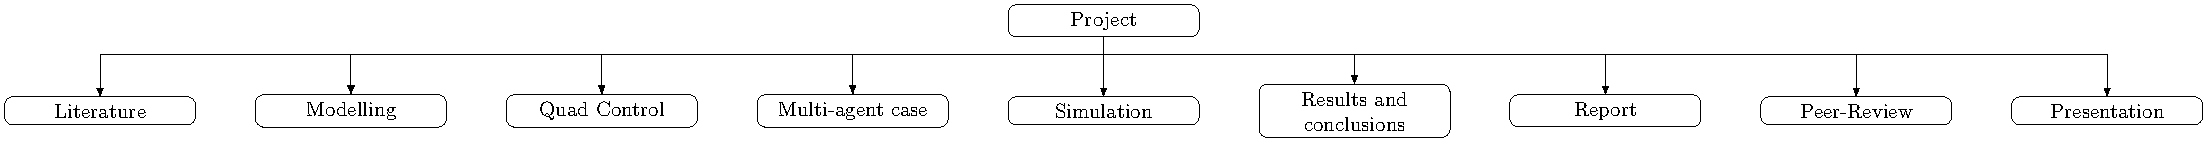
\includegraphics[width=1.15\linewidth]{Workplan_work_tree/basic_work_tree_diagram}
				\caption{Basic work tree}
				\label{fig:work_tree_basic}
		\end{figure}
		\begin{figure}[H]
			\centering
			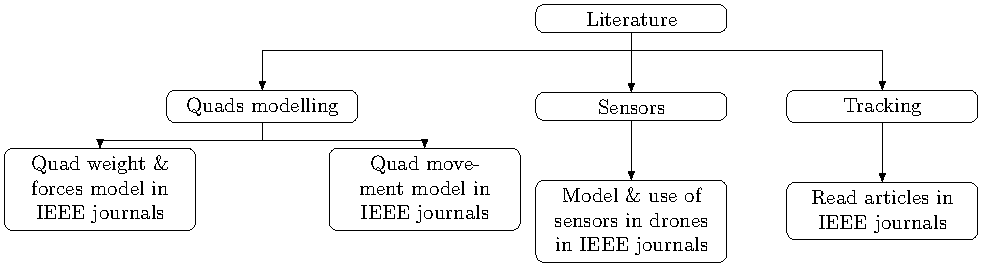
\includegraphics[width=.8\linewidth]{Workplan_work_tree/literature_work_tree_diagram}
			\caption{Expanded work tree for the literature section}
		\end{figure}
		\begin{figure}[H]
			\centering
			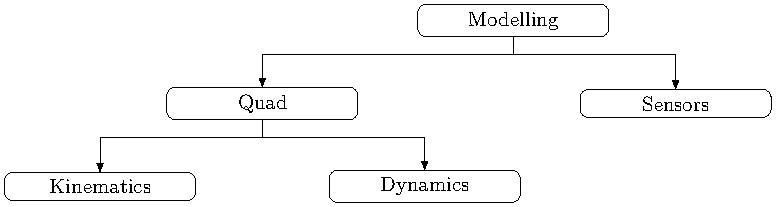
\includegraphics[width=.8\linewidth]{Workplan_work_tree/modelling_work_tree_diagram}
			\caption{Expanded work tree for the modelling section}
		\end{figure}
		\begin{figure}[H]
			\centering
			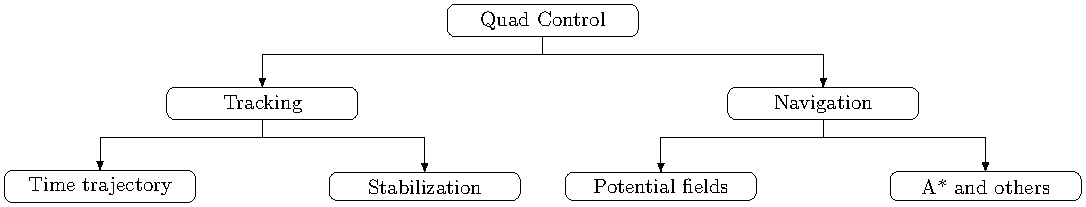
\includegraphics[width=.8\linewidth]{Workplan_work_tree/control_work_tree_diagram}
			\caption{Expanded work tree for the single-quad control section}
		\end{figure}
		\begin{figure}[H]
			\centering
			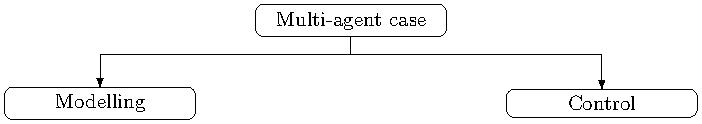
\includegraphics[width=.8\linewidth]{Workplan_work_tree/multiagent_work_tree_diagram}
			\caption{Expanded work tree for the multi-agent case section}
		\end{figure}
		\begin{figure}[H]
			\centering
			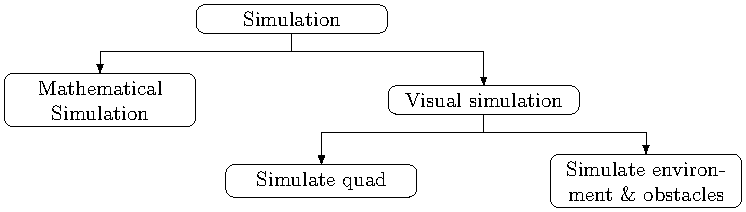
\includegraphics[width=.8\linewidth]{Workplan_work_tree/simulation_work_tree_diagram}
			\caption{Expanded work tree for the simulation section}
		\end{figure}
		
		\paragraph{} We will have a more detailed part of the simulation part of the work tree in status report 1 and a more detailed part of the report and peer-review part in status report 2.
		
			

	
	\section{Risk analysis}
		\begin{tabular}{|L {2.5cm}|C{0.3cm}|C{0.3cm}|C{0.3cm}|R{9.5cm}|}			
			Risks & P & C & R & Counter measure \\ \hline
			Diseases in the group  & 2 & 2 & 4 & Reactive: Rearrange workload \\ & & & & Proactive: Nothing \\ \hline
			Loss of documents and information & 2 & 4 & 8 & Reactive: recollect information again \\ & & & & Proactive: Have bakups for everything, use Google Drive and GitHub \\ \hline
			Running out of time & 4 & 2 & 8 & Reactive: Re-evaluate work plan and consult with supervisor \\ & & & & Proactive:  Have a good work plan, check on each other if we'll complete deadlines in time, check more when deadlines are closing in \\ \hline
			Bad communication with supervisor & 2 & 2 & 4 & Reactive: Send reminders if we get no answer in x amount of time. \\ & & & & Proactive: Schedule meetings now (once a week for example) and modify these dates if there is no need to meet. Ask supervisor how long 'x amount of time' should be. Plan accordingly\\ \hline
			Bad UAV Model & 3 & 3 & 9 & Reactive: Redesign UAV model?
			\\ & & & & Proactive: Test the calculated model with 3 individual tests of simple rotation and movement around and along one axis in a 3D space where the starting and final position is known either on paper or with matlab, check that you get the expected outcome. \\ \hline
			Bad sensor Model & & & & Reactive: %write something HERE! 
			\\ & & & & Proactive: \\ \hline
			Faulty state feedback controller & 4 & 3 & 12 & Reactive: Redesign the whole controller. damage control!\\ & & & & Proactive: Check the Observability, Controllability, Robustness Criteria and pole placement of the designed State feedback controller\\ \hline
			Potential Field/ A*-algorithm & & & & Reactive:\\
			& & & & Proactive:  \\ \hline %No idea what to write here, how to check if stuff goes haywire
			Multi-agent case & & & & Reactive:\\
			& & & & Proactive: \\ \hline
			Simulation & & & &  Reactive:\\
			& & & & Proactive: \\ \hline 
			      
		\end{tabular}		
 
	\section{Documentation/Communication rules}
	\begin{itemize}
			\item We will use Github and Google drive for documentation. MatLab, Latex and any other code will be stored on GitHub, and the rest will be stored on Google Drive.
			
			\item Meetings with supervisor are scheduled once a week, on Thursdays morning. The time and the confirmation for the next week are decided at the end of each meeting. In the case a meeting is cancelled, the designated responsible for communication with supervisor is in charge of scheduling another meeting for the next week or the week after. The purpose of these meetings is ask the supervisor questions or doubts, explain how the project is advancing, present goals accomplished in the case a section of the project plan is finished, check results and ask for how to improve them.
			
			\item Meetings with both students are not fixedly scheduled but regularly scheduled, at least once or twice a week depending on the availability of each one. The purpose of these meetings is advance on the project, distribute work to do for each section in the case the workload could be splitted, check the deadlines for the documents and make sure the work plan is being followed according to the planned schedule, and prepare questions for the supervisor in the case there was any.
			
			%anything else on this section?
	\end{itemize}

	
	\section{Appendix}
	
	\subsection{Time line}
		\begin{figure}[H]
			\centering
			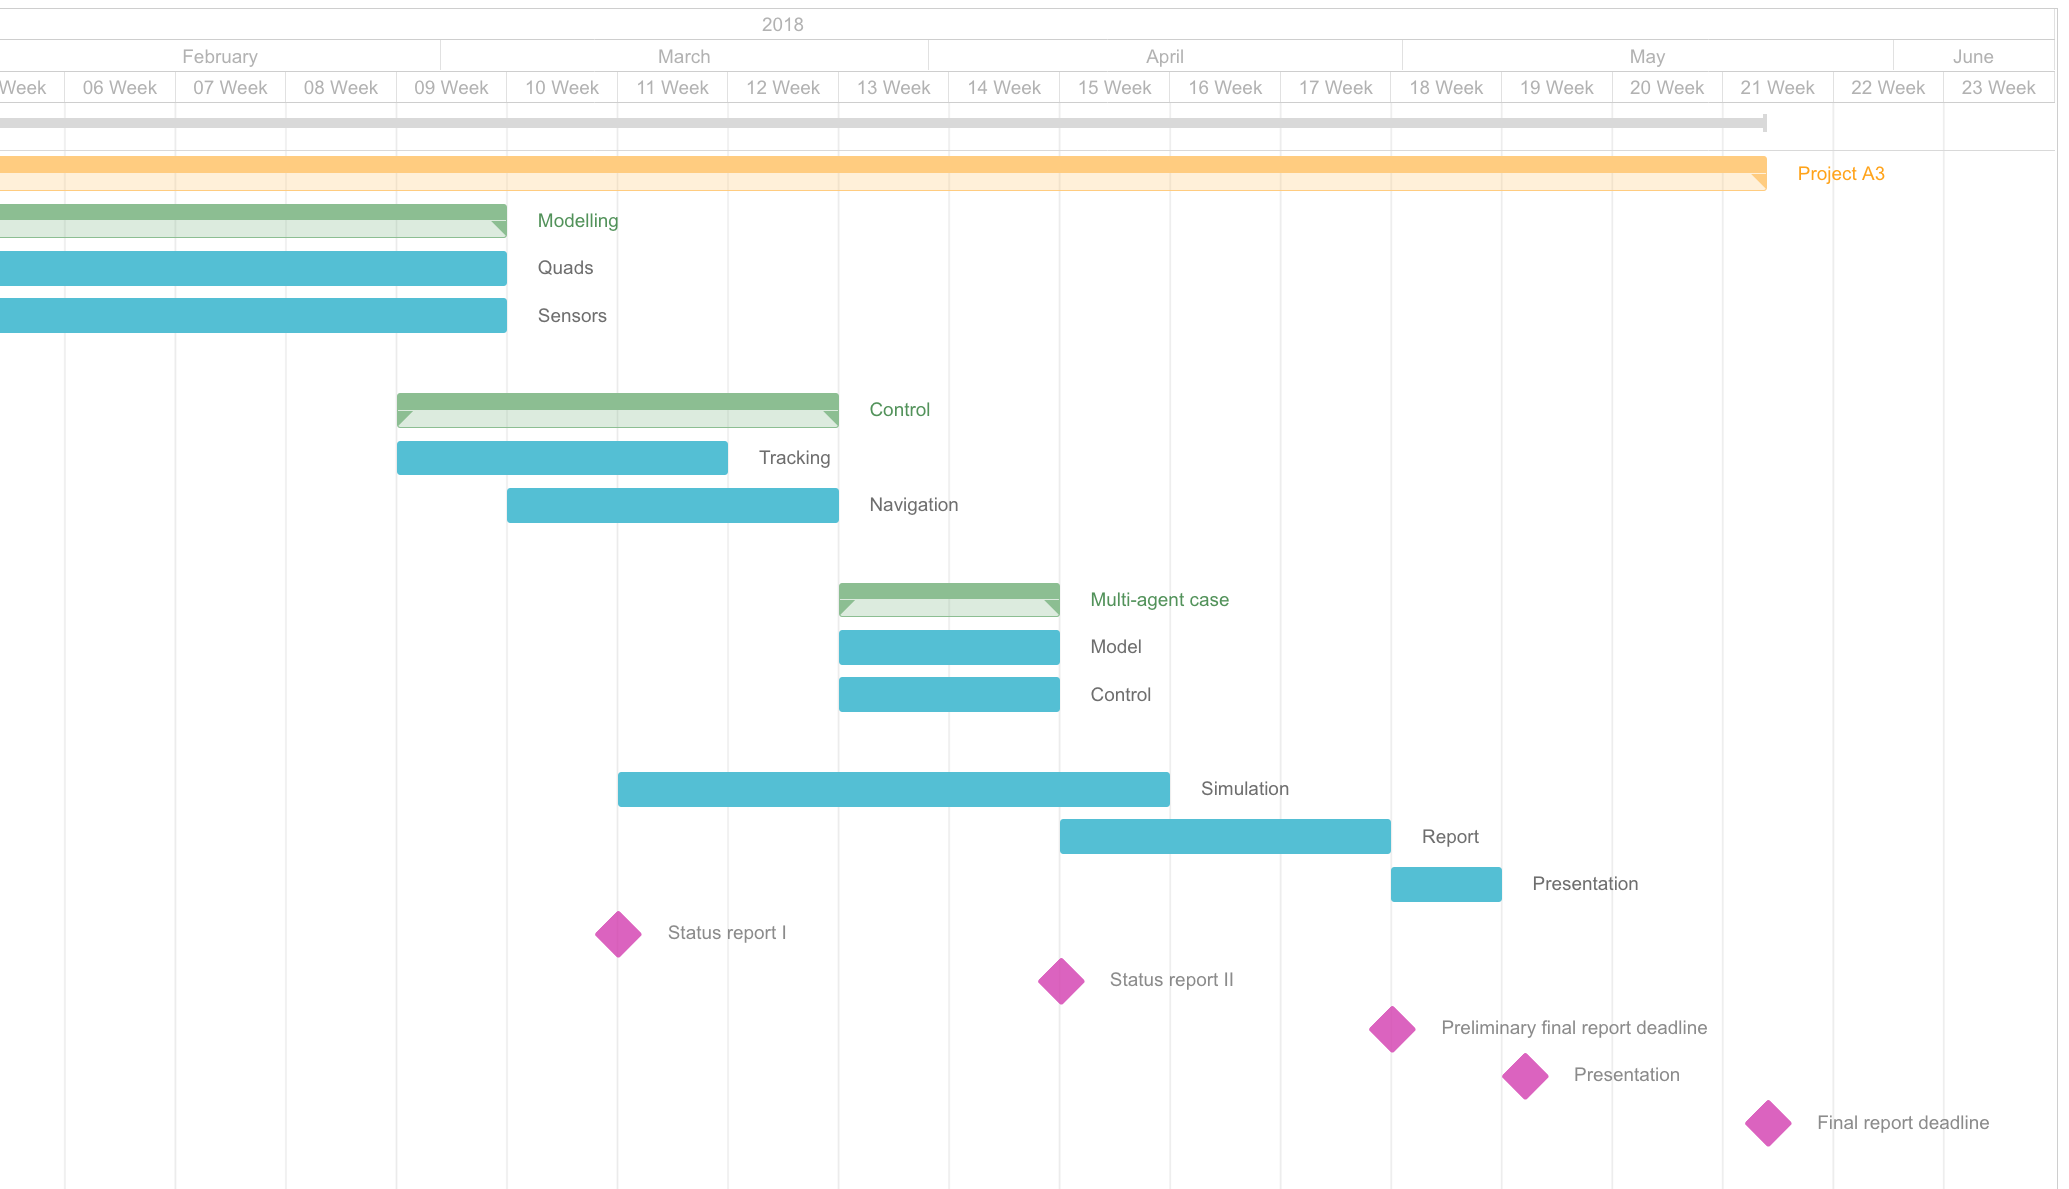
\includegraphics[width=\linewidth]{img/timeline}
			\caption{Time line for the project}
		\end{figure}
	\subsection{Resource plan}
\end{document}
